\documentclass[./../main.tex]{subfiles}
\graphicspath{{img/}}

\begin{document}
    \begin{exercise}
        ¿Qué tipo de acelerador es el LHC? ¿Se compone por más de un tipo? Explica el principio de su funcionamiento.

        \begin{solution}
            El LHC es un sincrotón que mide \SI{27}{\km} de circunferencia. Dentro de este dos haces de partículas a muy altas energía viajan a velocidades cercanas a la de la luz antes de colisionar. Los haces viajan en direcciones opuestas guiados mediante el uso electroimanes superconductores. 

            Los haces dentro del LHC colisionan en cuatros ubicaciones diferentes alrededor del anillo acelerador. En estas ubicaciones se encuentran los detectores ATLAS, CMS, ALICE y LHCb.

            El proceso de aceleración comienza con una fuente de haces de protones en el \emph{Linac4}, que acelera iones negativos de hidrógeno (\ch{H-}) a \SI{160}{\MeV} para prepararlo para su inyección en el \emph{Proton Synchrotron Booster} (PSB) o Impulsor del Sincrotón de Protones. Los electrones son despojados de sus dos electrones durante la inyección del \emph{Linac4} al PBS, dejando únicamente los protones. Estos son acelerados a \SI{2}{\GeV} para la inyección al \emph{Proton Synchrotron} (PS), el cual impulsa el haz hasta \SI{26}{\GeV}. Después los protones son enviados al \emph{Super Proton Synchrotron} (SPS), donde son acelerados hasta \SI{450}{\GeV}.

            Finalmente los protones son transferidos a las dos tuberías especiales para que viajen los haces. La primera tubería circula en dirección de las manecillas del reloj, mientras que el haz en la otra tubería circula en sentido contrario a las manecillas del reloj. Los haces entonces se hacen colisionar dentro de los cuatro detectores antes mencionados, de tal manera que la energía total en el punto de colisión es de \SI{13}{\TeV}.

            \begin{figure}[htb]
                \centering
                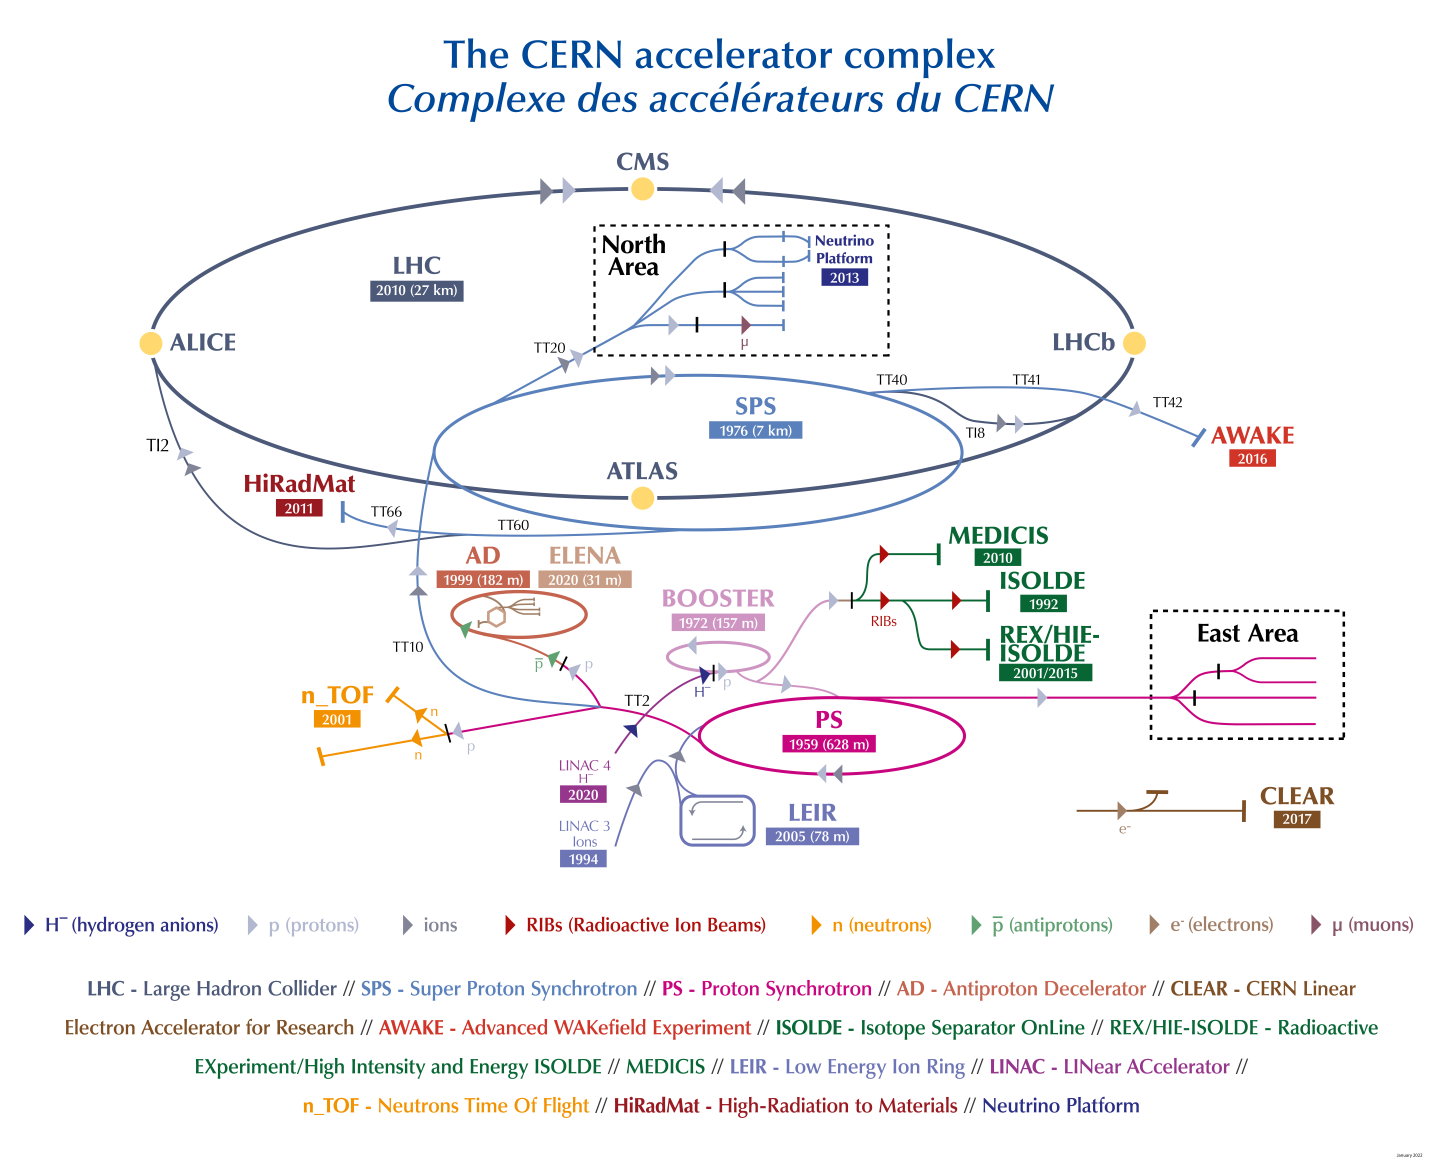
\includegraphics[scale=0.9]{lhc}
                \caption{Diagrama del LHC con cada uno de sus componentes. \parencite{LHCComplex}}
                \label{fig:LHC}
            \end{figure}
        \end{solution}
    \end{exercise}
\end{document}